\section{Results}\label{sec6}
\begin{itemize}
\item Simulating a positive one standard deviation productivity shock on the agricultural sector:
\end{itemize}


\begin{figure}[H]
\centering
\begin{tabular}{c}
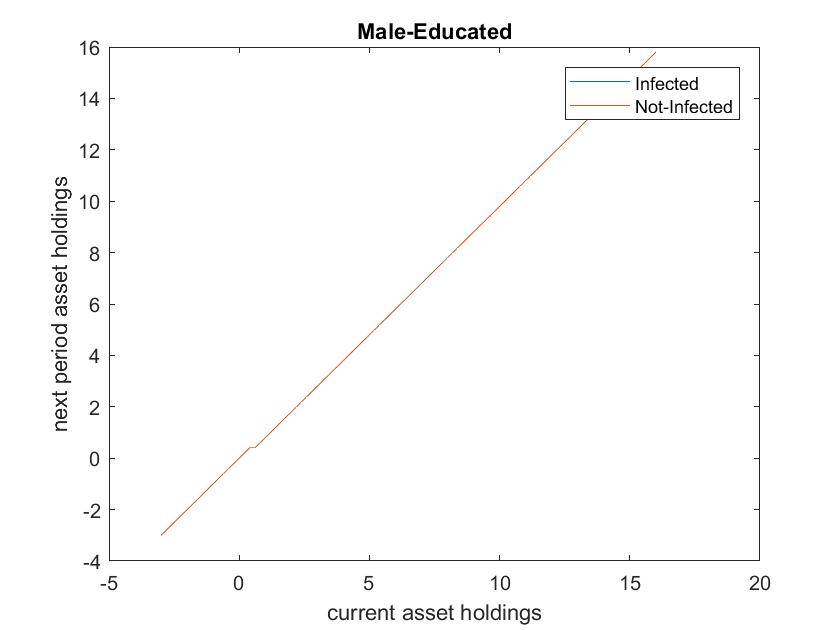
\includegraphics[width = 1\textwidth, height = 0.4\textheight]{sections/fig1.jpg}\\
\end{tabular}
\caption{Impulse response function on aggregate variables}
\label{fig1}
\end{figure}

\begin{figure}[H]
\centering
%\includegraphics[width = 15cm, height = 11cm]{sections/fig_t.jpg}\\
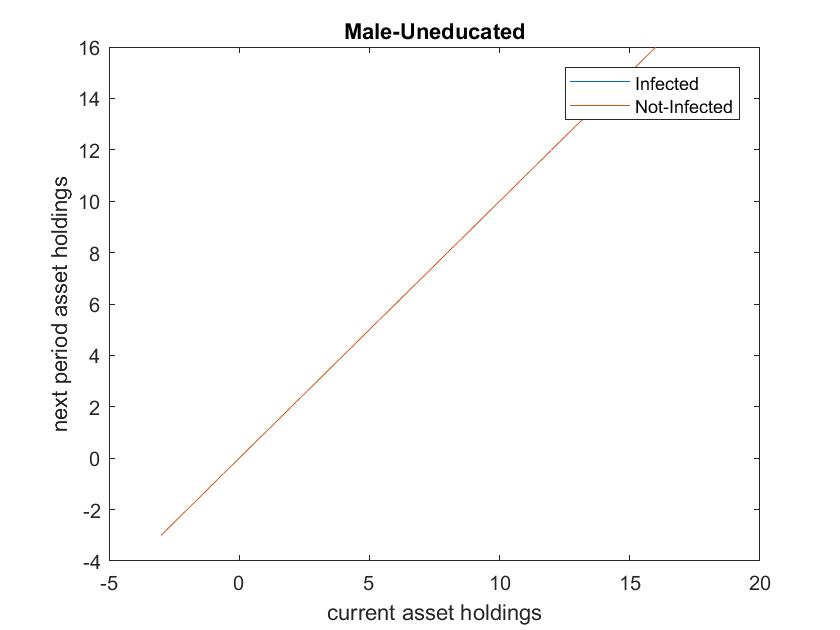
\includegraphics[width = 1\textwidth, height = 0.4\textheight]{sections/fig2.jpg}\\

\caption{Impulse response function on the agricultural sector}
\label{fig2}
\end{figure}

\begin{figure}[H]
\centering
%\begin{tabular}{c}
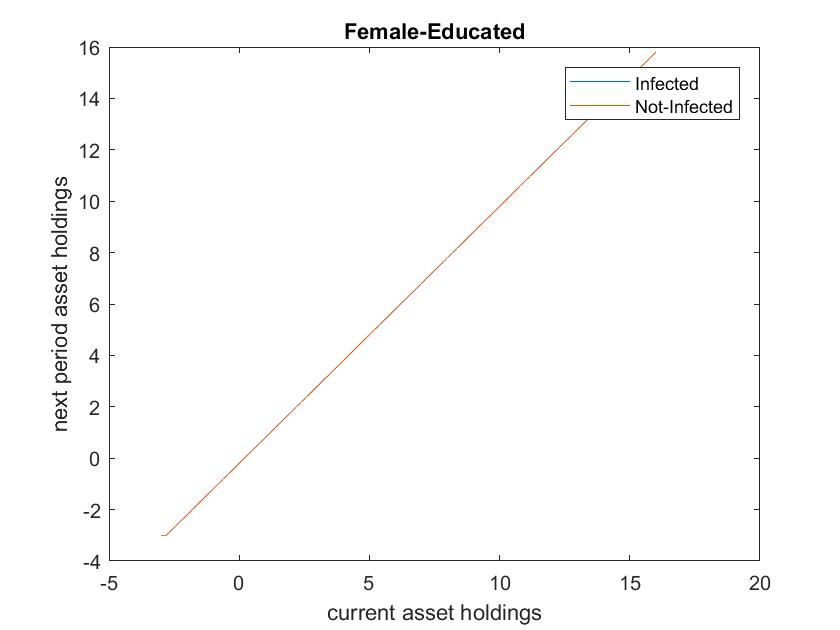
\includegraphics[width = 1\textwidth, height = 0.4\textheight]{sections/fig3.jpg}\\
%\end{tabular}
\caption{Impulse response function on the industry sector}
\label{fig3}
\end{figure}

\begin{figure}[H]
\centering
%\begin{tabular}{c}
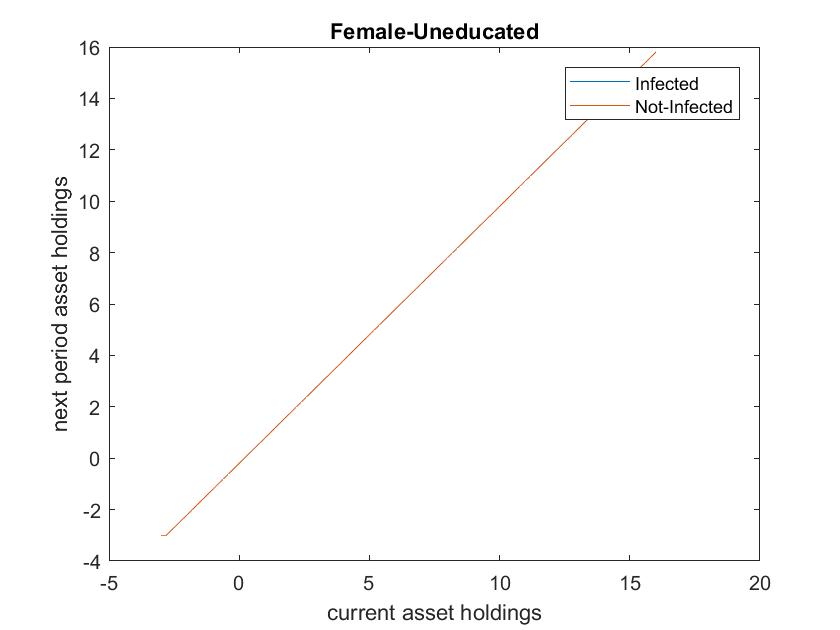
\includegraphics[width = 1\textwidth, height = 0.4\textheight]{sections/fig4.jpg}\\
%\end{tabular}
\caption{Impulse response function on the services sector}
\label{fig4}
\end{figure}

It can be seen in Figure\ref(fig2) that a positive shock on the agricultural sector, increases agricultural production and with it internal demand for inputs (co-movement) in addition the effect remains for at least two periods in the future(persistence)\footnote{it is important to note that the persistence in the model occurs by construction do to the high value of the shock auto-correlation parameter, if $\rho_{k}=0$ persistence is no longer observable}. Figure \ref{fig1} shows that the increase of agricultural production leads to an increase of total production in the economy, however, unemployment rises because employees from less productive sectors loose their jobs and are not immediately allocated to the more productive sector due to training costs.  Furthermore, an increase of the productivity in one sector will attract employment to the high productive sector, reducing the amount of people employed on the other industries, this is the case for the industry and services sector, see Figure\ref{fig3}, Figure\ref{fig4}. These results are broadly consistent with the findings in the literature on sectoral analysis \cite{long}, \cite{basu}, \cite{santoro}.

\section{Concluding Remarks}\label{conclu}
The Model presented in the following sections lacks micro-economic foundations for the inclusion of the price ratios. It therefore compulsory to switch into to a specification in which these are justified. 
The calculation of the steady state of model is extremely sensitive to slight changes in the parametrization, as the solution routine requires to input values that are close to the solution.

